%\VignetteIndexEntry{QTLBIM Prototype Slides Analyzing Hyper Data}
%\VignetteDepends{qtlbim}
%\VignetteKeywords{QTL}
%\VignettePackage{qtlbim}
\documentclass{beamer}

\usepackage{beamerthemesplit}

\usepackage{Sweave}

\begin{document}





\title{Prototype QTL Strategy: Phenotype
bp
in Cross
hyper}
\author{Brian S. Yandell, W. Whipple Neely, Nengjun Yi}
\date{\today}

\frame{\titlepage}

\section[Outline]{}
\frame{\tableofcontents}

\section{Overview}

\frame
{
  \frametitle{Automated Strategy}

  \begin{itemize}
  \item Estimate positions and effects of main QTL.
  \item Find chromosomes with epistasis.
  \item Estimate epistatic pair positions and effects.
  \item Confirm genetic architecture with ANOVA.
  \end{itemize}
}

\begin{frame}[fragile]
  \frametitle{Running Sweave}


\tiny

\begin{Schunk}
\begin{Sinput}
> library(qtlbim)
\end{Sinput}
\end{Schunk}
\begin{Schunk}
\begin{Sinput}
> qb.sweave(hyper, pheno.col = 1,
+  n.iter = 3000, n.draws = 8,
+  scan.type = "2logBF", hpd.level = 0.5,
+  threshold = c(upper = 2),
+  SweaveFile = "/tmp/Rinst2188206948/qtlbim/doc/hyperslide.Rnw",
+  SweaveExtra = "/tmp/Rinst2188206948/qtlbim/external/hyperslideextra.Rnw",
+  PDFDir = "bpPDF",
+  remove.qb = TRUE)
\end{Sinput}
\end{Schunk}

\end{frame}

\subsection{Initialization}

\begin{frame}[fragile]
  \frametitle{Cross Object}

\tiny

\begin{Schunk}
\begin{Sinput}
> summary(cross)
\end{Sinput}
\begin{Soutput}
    Backcross

    No. individuals:    250 

    No. phenotypes:     2 
    Percent phenotyped: 100 100 

    No. chromosomes:    19 
        Autosomes:      1 2 3 4 5 6 7 8 9 10 11 12 13 14 15 16 17 18 19 

    Total markers:      170 
    No. markers:        22 8 6 20 14 11 7 6 5 5 14 5 5 5 11 6 12 4 4 
    Percent genotyped:  47.9 
    Genotypes (%):      AA:50.1  AB:49.9 
\end{Soutput}
\end{Schunk}

\end{frame}

\begin{frame}[fragile]
  \frametitle{Create MCMC runs}

\tiny

\begin{Schunk}
\begin{Sinput}
> cross <- qb.genoprob(cross,step=2)
> cross.qb <- qb.mcmc(cross, pheno.col = pheno.col,
+   genoupdate=TRUE, n.iter = 3000, verbose=FALSE)
\end{Sinput}
\end{Schunk}

\end{frame}

\section{1-D \& 2-D Scans}

\begin{frame}[fragile]
  \frametitle{1-D 2logBF Scan}

\tiny

\begin{Schunk}
\begin{Sinput}
> hpd.level
\end{Sinput}
\begin{Soutput}
[1] 0.5
\end{Soutput}
\begin{Sinput}
> scan.type
\end{Sinput}
\begin{Soutput}
[1] "2logBF"
\end{Soutput}
\begin{Sinput}
> cross.hpd <- qb.hpdone(cross.qb, hpd.level, scan.type)
> sum.one <- summary(cross.hpd)
> sum.one
\end{Sinput}
\begin{Soutput}
   chr n.qtl  pos lo.50% hi.50% 2logBF       A       H
1    1 0.829 64.5   64.5   72.1  6.692 103.611  99.090
4    4 3.228 29.5   25.1   31.7 11.169 104.584  98.020
6    6 1.033 59.0   56.8   66.7  6.054  99.637 102.965
15  15 0.159 17.5   17.5   17.5  5.837 101.972 100.702
\end{Soutput}
\begin{Sinput}
> chrs <- as.vector(sum.one[, "chr"])
> pos <- sum.one[, "pos"]
\end{Sinput}
\end{Schunk}
\begin{Schunk}
\begin{Sinput}
> plot(cross.hpd)
\end{Sinput}
\end{Schunk}

\end{frame}

\begin{frame}[fragile]
  \frametitle{1-D Scan: 2logBF Profile}

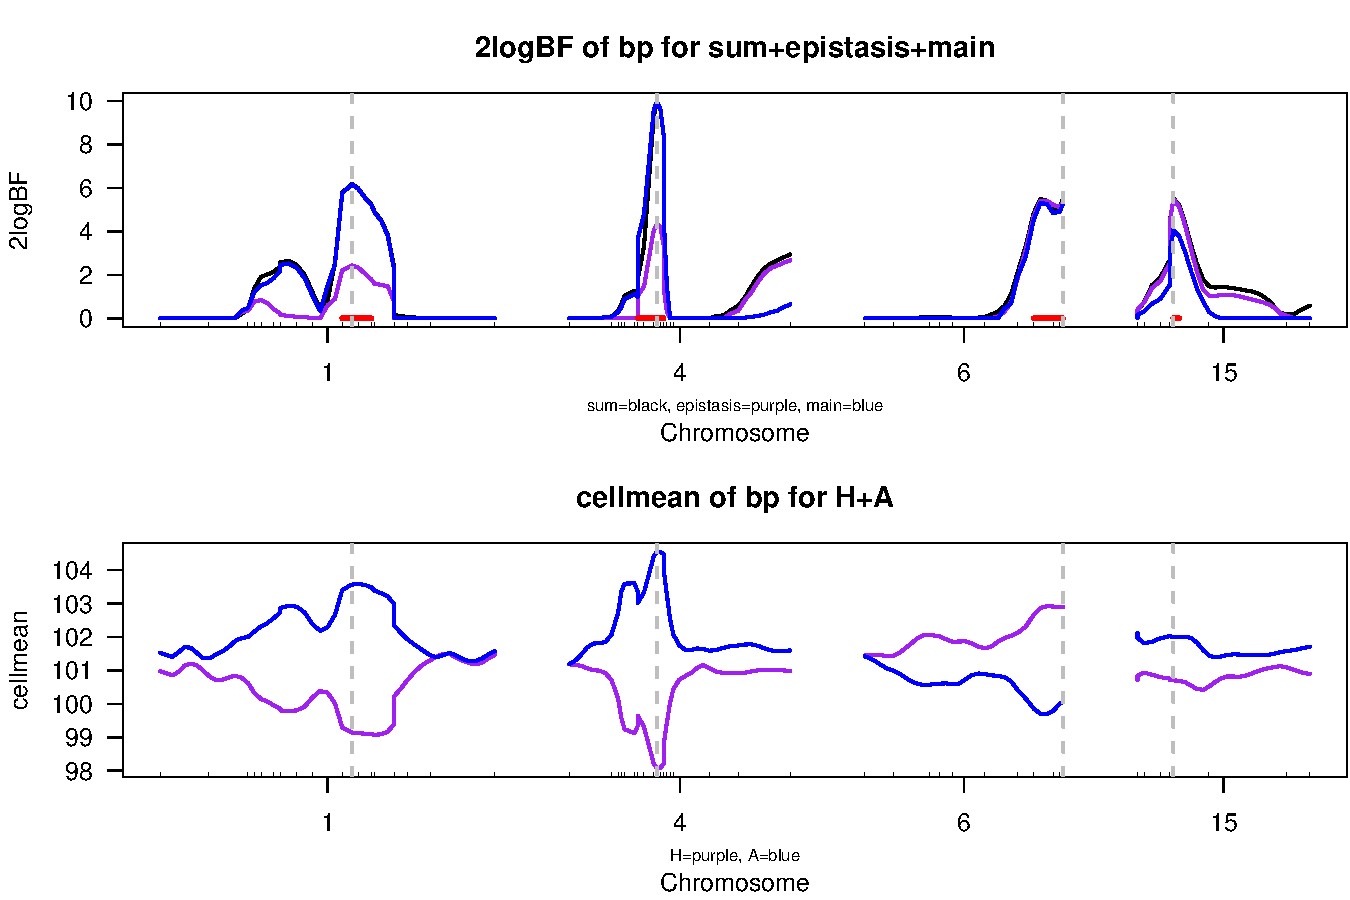
\includegraphics{bpPDF/slide1hpd.pdf}
\end{frame}

\begin{frame}[fragile]
  \frametitle{2-D: find epistatic pairs}

\tiny

\begin{Schunk}
\begin{Sinput}
> two <- qb.scantwo(cross.qb, chr = chrs, type = scan.type)
> sum.two <- summary(two, sort = "upper", threshold = threshold, 
+     refine = TRUE)
> sum.two
\end{Sinput}
\begin{Soutput}
upper: 2logBF of bp for epistasis
lower: 2logBF of bp for full 
Thresholds: upper=2 

        n.qtl l.pos1 l.pos2 lower u.pos1 u.pos2 upper
c6 :c15 1.004   59.0   17.5 12.53   59.0   17.5 12.50
c4 :c6  1.452   29.5   59.0 14.58   74.3   59.0  7.84
c4 :c15 0.417   29.5   17.5 14.27   74.3   47.6  7.00
c15:c15 0.111   17.5   33.5  7.66   17.5   31.5  6.61
c1 :c4  1.255   67.8   29.5 15.51   72.1   29.5  6.37
c1 :c6  1.817   67.8   66.7 12.05   67.8   59.0  5.43
c1 :c15 0.261   67.8   17.5 11.71   72.1   17.5  5.40
c1 :c1  0.366   37.2   77.6  7.94   39.4   77.6  5.23
c4 :c4  1.103   29.5   74.3 11.47   28.4   49.5  4.76
c6 :c6  1.185   61.2   65.6  7.70   40.4   56.8  3.94
\end{Soutput}
\end{Schunk}

\end{frame}

\begin{frame}[fragile]
  \frametitle{Initial Genetic Architecture}

\tiny

\begin{Schunk}
\begin{Sinput}
> cross.arch <- qb.arch(sum.two, chrs, pos)
> cross.arch
\end{Sinput}
\begin{Soutput}
main QTL loci:
        1     2     3     4    5    6     7    8     9    10
chr  1.00  1.00  4.00  4.00  4.0  6.0  6.00 15.0 15.00 15.00
pos 39.35 70.82 29.13 49.45 74.3 40.4 58.56 17.5 31.52 47.64

Epistatic pairs by qtl, chr, pos:
   qtla qtlb chra chrb  posa  posb
1     7    8    6   15 58.56 17.50
2     5    7    4    6 74.30 58.56
3     5   10    4   15 74.30 47.64
4     8    9   15   15 17.50 31.52
5     2    3    1    4 70.82 29.13
6     2    7    1    6 70.82 58.56
7     2    8    1   15 70.82 17.50
8     1    2    1    1 39.35 70.82
9     3    4    4    4 29.13 49.45
10    6    7    6    6 40.40 58.56
Epistatic chromosomes by connected sets:
1,4,6,15 
\end{Soutput}
\end{Schunk}

\end{frame}
 
\section{Anova Fit}

\begin{frame}[fragile]
  \frametitle{Construct QTL Object}

\tiny

use R/qtl tools to check model fit\\
first simulate missing markers\\
then construct QTL object

\begin{Schunk}
\begin{Sinput}
> cross.sub <- subset(cross, chr = unique(cross.arch$qtl$chr))
> n.draws
\end{Sinput}
\begin{Soutput}
[1] 8
\end{Soutput}
\begin{Sinput}
> cross.sub <- sim.geno(cross.sub, n.draws = n.draws, step = 2, 
+     error = 0.01)
> qtl <- makeqtl(cross.sub, cross.arch$qtl$chr, cross.arch$qtl$pos)
> cross.sub <- clean(cross.sub)
\end{Sinput}
\end{Schunk}
\end{frame}

\begin{frame}[fragile]
  \frametitle{Stepwise Reduction}

\tiny

\begin{Schunk}
\begin{Sinput}
> cross.step <- step.fitqtl(cross.sub, qtl, pheno.col, cross.arch)
\end{Sinput}
\begin{Soutput}
   drop                  LOD    p     
1  Chr1@39.35:Chr1@70.82 0.0764 0.5710
2  Chr4@29.13:Chr4@49.45 0.2280 0.3260
3  Chr1@70.82:Chr6@58.56 0.3080 0.2530
4  Chr1@70.82:Chr15@17.5 0.3800 0.2030
5  Chr6@40.4:Chr6@58.56  0.4130 0.1830
6  Chr6@40.4             0.3890 0.1960
7  Chr4@49.45            0.4700 0.1540
8  Chr4@74.3:Chr15@47.64 0.5520 0.1220
9  Chr1@39.35            0.2920 0.2590
10 Chr15@47.64           0.8140 0.0591
11 Chr1@70.82:Chr4@29.13 0.8220 0.0573
\end{Soutput}
\end{Schunk}
\begin{Schunk}
\begin{Sinput}
> summary(cross.step$fit)
\end{Sinput}
\end{Schunk}
\begin{Schunk}
\begin{Soutput}
       df        SS        MS      LOD     %var Pvalue(Chi2) Pvalue(F)
Model   9  6713.682 745.96463 25.94849 37.99709            0         0
Error 240 10955.255  45.64689                                         
Total 249 17668.936                                                   
\end{Soutput}
\end{Schunk}
\end{frame}

\begin{frame}[fragile]
\frametitle{Stepwise Reduction}

\tiny

\begin{Schunk}
\begin{Soutput}
                       df Type III SS      LOD     %var F value Pvalue(F)    
Chr1@70.82              1    1430.826    6.664    8.098  31.346  5.89e-08 ***
Chr4@29.13              1    2505.998   11.183   14.183  54.900  2.15e-12 ***
Chr4@74.3               2     700.002    3.362    3.962   7.668  0.000592 ***
Chr6@58.56              3    1853.558    8.486   10.490  13.535  3.45e-08 ***
Chr15@17.5              3    1728.599    7.954    9.783  12.623  1.09e-07 ***
Chr15@31.52             2     360.360    1.757    2.040   3.947  0.020574 *  
Chr6@58.56:Chr15@17.5   1    1146.912    5.405    6.491  25.126  1.04e-06 ***
Chr4@74.3:Chr6@58.56    1     471.825    2.289    2.670  10.336  0.001483 ** 
Chr15@17.5:Chr15@31.52  1     364.857    1.779    2.065   7.993  0.005092 ** 
\end{Soutput}

\end{Schunk}
\end{frame}
\begin{frame}[fragile]
  \frametitle{Reduced Genetic architecture}

\tiny

\begin{Schunk}
\begin{Sinput}
> cross.arch <- cross.step$arch
> cross.arch
\end{Sinput}
\begin{Soutput}
main QTL loci:
        2     3    5     7    8     9
chr  1.00  4.00  4.0  6.00 15.0 15.00
pos 70.82 29.13 74.3 58.56 17.5 31.52

Epistatic pairs by qtl, chr, pos:
  q1 q2 chra chrb  posa  posb
1  7  8    6   15 58.56 17.50
2  5  7    4    6 74.30 58.56
3  8  9   15   15 17.50 31.52
Epistatic chromosomes by connected sets:
4,6,15 
\end{Soutput}
\end{Schunk}
\end{frame}

\begin{frame}[fragile]
  \frametitle{2-D Plots}

2-D plots by cliques (if any epistasis)

\tiny

\begin{Schunk}
\begin{Sinput}
> for(i in names(cross.arch$chr.by.set))
+   plot(two, chr = cross.arch$chr.by.set[[i]], smooth = 3,
+     col = "gray", contour = 3)
\end{Sinput}
\end{Schunk}

\end{frame}

\begin{frame}[fragile]
\frametitle{2-D Plots: clique 1 }

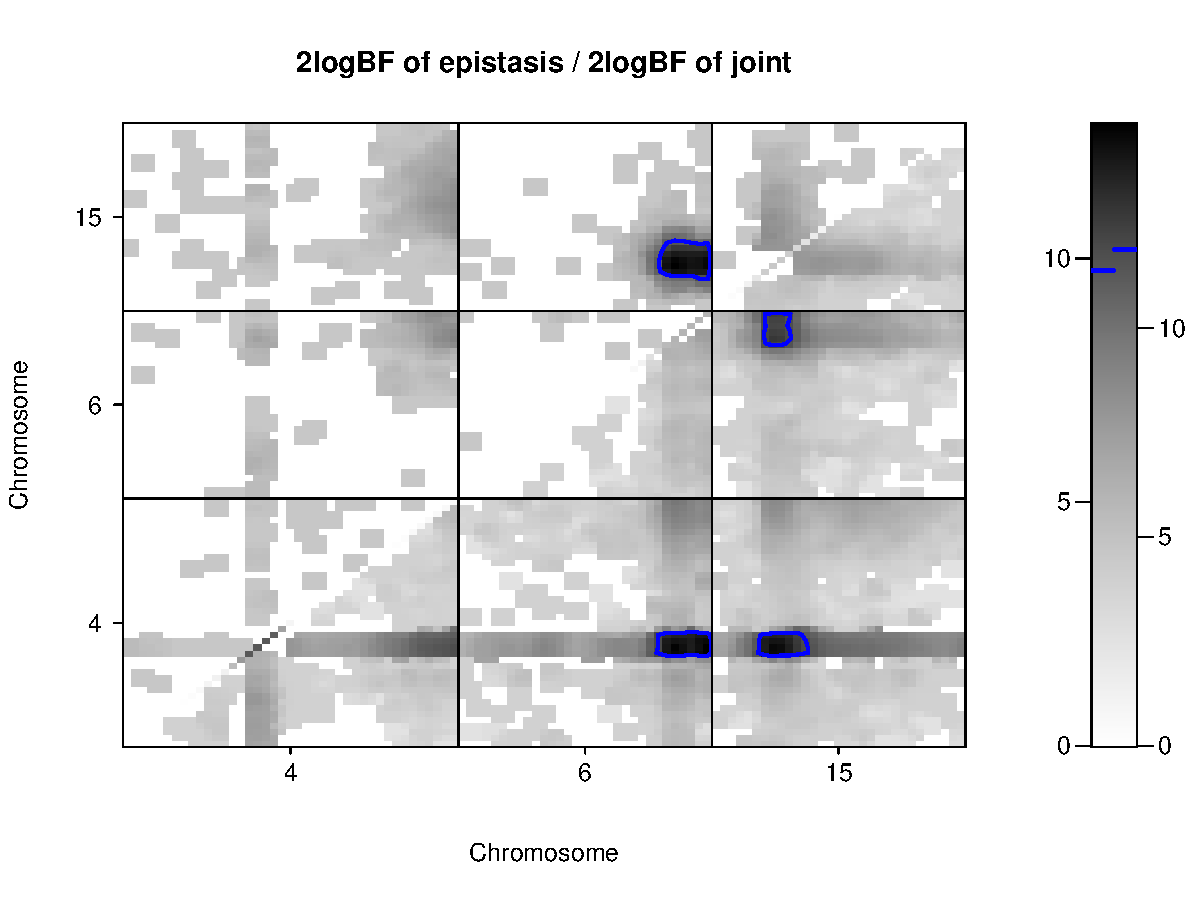
\includegraphics{bpPDF/slide2LOD-1.pdf}


\end{frame}
\begin{frame}[fragile]
  \frametitle{Slice Each Epistatic Pair}

show detail plots for epistatic pairs (if any)

\tiny

\begin{Schunk}
\begin{Sinput}
> if(!is.null(cross.arch$pair.by.chr)) {
+  for(i in seq(nrow(cross.arch$pair.by.chr$chr))) {
+    chri <- cross.arch$pair.by.chr$chr[i,]
+    posi <- cross.arch$pair.by.chr$pos[i,]
+    if(chri[1] != chri[2])
+      plot(qb.slicetwo(cross.qb, chri, posi, scan.type))
+  }
+}
\end{Sinput}
\end{Schunk}

\end{frame}


\begin{frame}[fragile]
\frametitle{Epistatic Pair 6 and 15 }

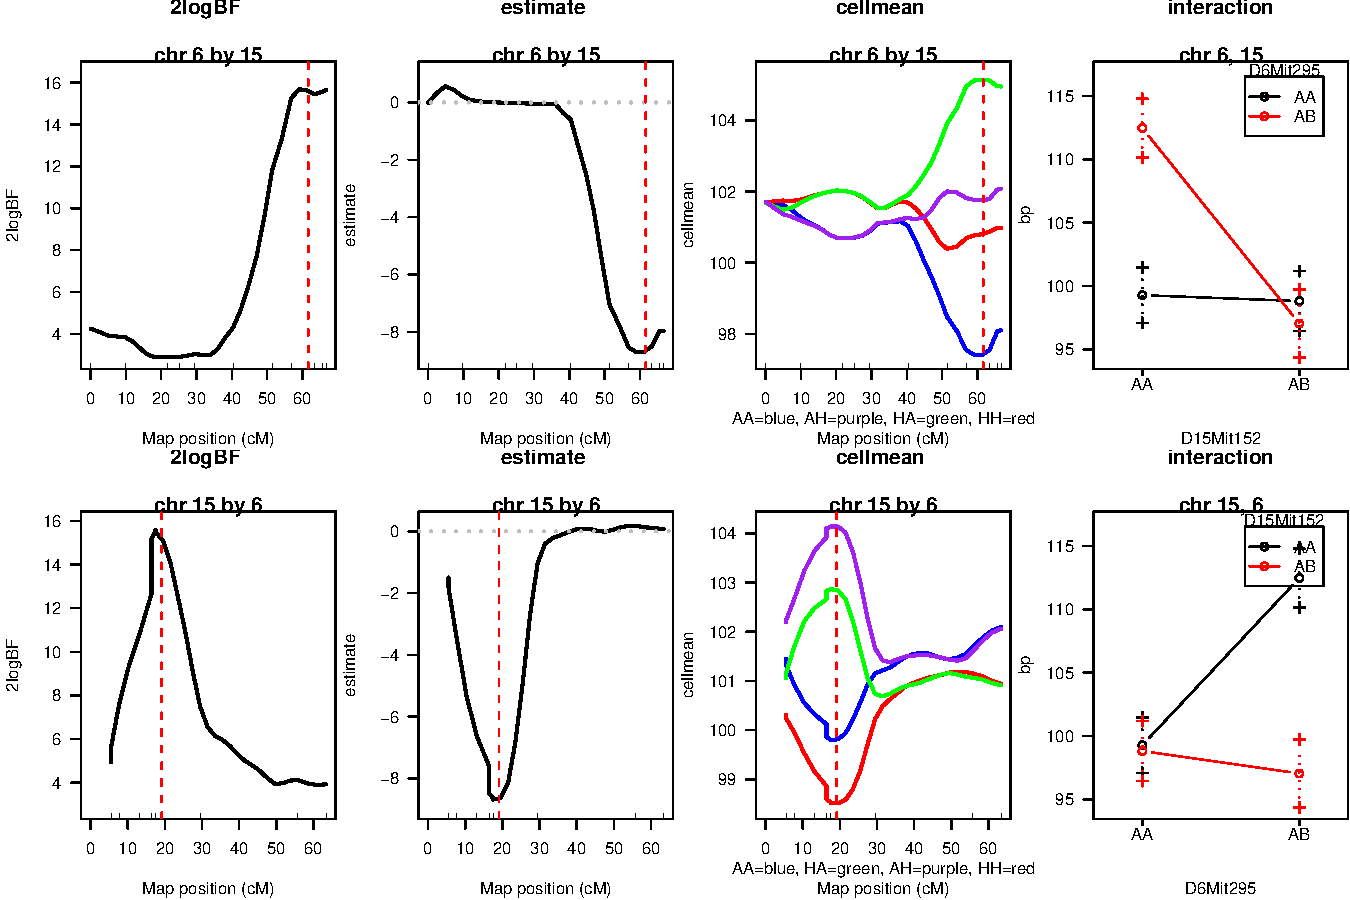
\includegraphics{bpPDF/slide-6-15.pdf}


\end{frame}

\begin{frame}[fragile]
\frametitle{Epistatic Pair 4 and 6 }

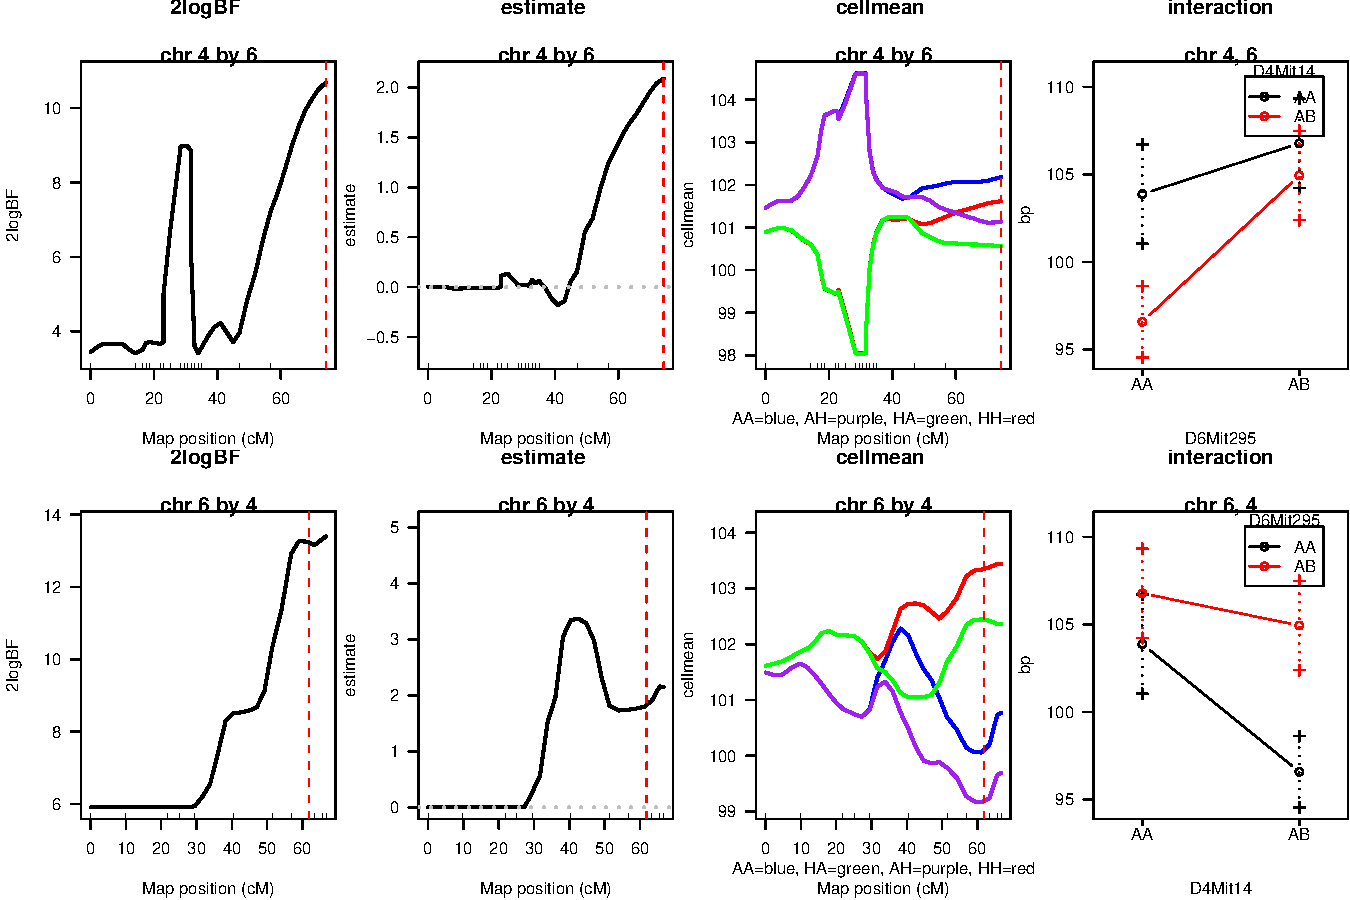
\includegraphics{bpPDF/slide-4-6.pdf}


\end{frame}
% \VignetteIndexEntry{QTLBIM Prototype Slides: User Customized Section}
% \VignetteDepends{qtlbim}
% \VignetteKeywords{QTL}
%\VignettePackage{qtlbim}



\section{User Customized Section}

\begin{frame}[fragile]
  \frametitle{Compare with Literature}

\tiny

Sugiyama et al. (2002) found:\\
two main QTLs on 1 4\\
two epistatic pairs with 6.15, 7.15

compare to present model:

\begin{Schunk}
\begin{Sinput}
> arch3 <- qb.arch(cross.step, main = c(1, 4), epistasis = data.frame(q1 = c(6, 
+     7), q2 = rep(15, 2)))
> arch3
\end{Sinput}
\end{Schunk}

\end{frame}

\begin{frame}[fragile]
  \frametitle{Sugiyama Model}

\tiny

\begin{Schunk}
\begin{Sinput}
> cross.step2 <- step.fitqtl(cross.sub, qtl, pheno.col, arch3)
\end{Sinput}
\end{Schunk}
\begin{Schunk}
\begin{Sinput}
> summary(cross.step2$fit)
\end{Sinput}
\end{Schunk}
\end{frame}


\begin{frame}[fragile]
  \frametitle{Sugiyama vs. Automata}

formal comparison with automated model

\tiny

\begin{Schunk}
\begin{Sinput}
> anova(cross.step, cross.step2)
\end{Sinput}
\end{Schunk}

\end{frame}


\section{Conclusion}

\begin{frame}[fragile]

final tasks:\\
externally rename file hyperslide.tex to bp.tex\\
and run pdflatex twice on it\\
remove objects created by {\tt R/qtlbim} if desired

\tiny

\begin{Schunk}
\begin{Sinput}
> file.rename("hyperslide.tex", "bp.tex")
> invisible(system("pdflatex bp.tex",intern=TRUE))
> invisible(system("pdflatex bp.tex",intern=TRUE))
\end{Sinput}
\end{Schunk}
\begin{Schunk}
\begin{Sinput}
> remove.qb
\end{Sinput}
\begin{Soutput}
[1] FALSE
\end{Soutput}
\begin{Sinput}
> if (remove.qb) {
+     qb.remove(cross.qb)
+     rm(cross, cross.sub, pheno.col, threshold, n.iter, n.draws, 
+         remove.qb)
+ }
\end{Sinput}
\end{Schunk}


\end{frame}

\end{document}
